\documentclass{astroedu-lab}

\begin{document}

\pagestyle{plain}

\begin{problem}{\huge Лабораторная работа 4.5.2\\\\Интерференция лазерного излучения\\\\Выполнил Жданов Елисей Б01-205}

\section{Цель работы:}

Исследование видности интерференционной картины излучения гелий-неонового лазера и определение длины когерентности излучения.

\section{Оборудование:}

Не–Nе лазер

Интерферометр Майкельсона с подвижным зеркалом

Фотодиод с усилителем

Осциллограф

Поляроид

Линейка

\section{Теоретическая справка}

\paragraph*{Гелий-неоновый лазер}
Лазер представляет собой интерферометр Фабри-Перо -- газовую трубку с двумя параллельными зеркалами по обе стороны. Пусть $\Delta F$ -- половина диапазона генерации лазера, а $\Delta \nu$ -- межмодовое расстояние. Тогда межмодовое расстояние выражается как
\begin{equation}
    \Delta \nu = \dfrac{c}{2L}
\end{equation}
При этом число мод можно оценить как 
\begin{equation}
N \approx 1 + \dfrac{2\Delta F}{\Delta \nu}.
\end{equation}
\paragraph*{Видимость}
Видимость интерфереционной картины -- параметр, определяемый формулой
\begin{equation}
\gamma = \dfrac{I_{max} - I_{min}}{I_{max} + I_{min}},
\end{equation}
где $I_{max}$, $I_{min}$ -- максимальная и минимальная интенсивности света интерфереционной картины вблизи выбранной точки. Разобьём его на произведение функций параметров установки
$$
\gamma = \gamma_1 \gamma_2 \gamma_3.
$$
Здесь $\gamma_1$
\begin{equation}
\gamma_1 = \dfrac{2\sqrt{\delta}}{1+\delta},
\end{equation}
где $\delta = \frac{B_m^2}{A_m^2}$, $A_m^2$ и $B_m^2$ -- интенсивности волн. Параметр $\delta$ выражает отношение интенсивностей интерферирующих волн.\\
Величина $\gamma_2$ зависит от геометрической разности хода интерферирующих волн,
$$
\gamma_2 = \dfrac{\sum\limits_n A^2_n \cos \frac{2\pi \Delta \nu n l}{c}}{\sum\limits_n A_n^2},
$$
где $l$ -- разность хода, $\Delta \nu$ -- спектральный состав излучения, $A_n^2$ -- интенсивности мод. 
\begin{figure}[H]
\begin{center}
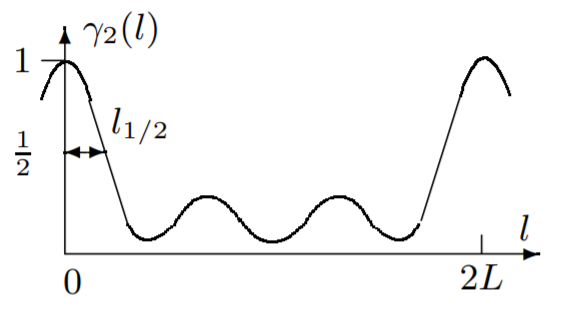
\includegraphics[scale=0.6]{1.png}
\end{center}
\caption{Зависимость $\gamma_2(l)$.}
\end{figure}
\noindent Приблизим $\gamma_2$ вблизи максимума
$$
\gamma_2 = e^{-\left(\frac{\pi \Delta F l}{c}\right)^2}
$$
Таким образом, ма имеем гауссову зависимость видности от разности хода $\gamma_2(l)$ с полушириной 
\begin{equation}
l_{1/2} = \dfrac{c}{\pi \Delta F}\sqrt{\ln 2} \approx \dfrac{0.26 c}{\Delta F}.
\end{equation}
Величина $\gamma_3$ соответсвует тому факту, что при интерференции поляризованных волн интерфирируют лишь компоненты, поляризованные одинкаово. ПУсть $\alpha$ -- угол между плоскостями поляризаций волн, тогдв
\begin{equation}
\gamma_3 = |\cos \alpha|.
\end{equation}

\section{Экспериментальная установка}

\begin{figure}[!h]
	\centering
	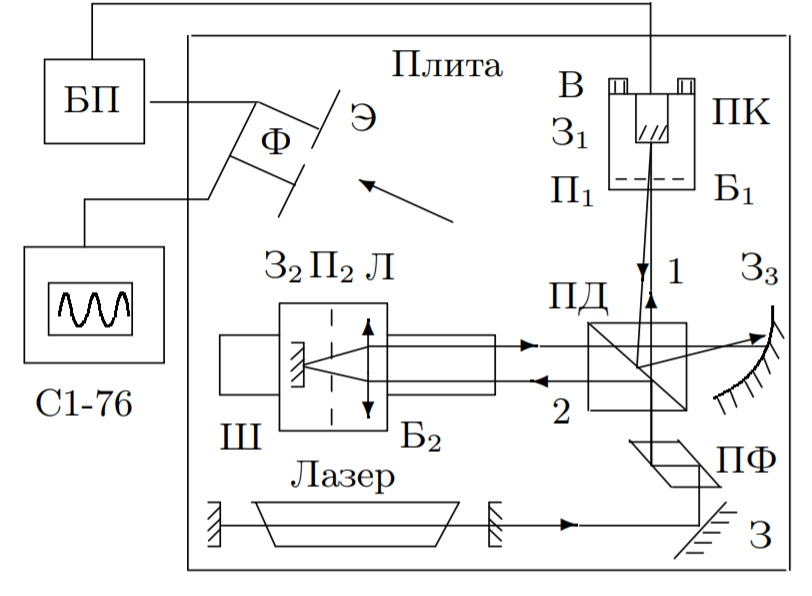
\includegraphics[width=0.5\textwidth]{2.png}
	\label{fig:boiler}
\end{figure}

В работе используется интерферометр Майкельсона, схема работы которого представлена на рис. 2. При этом для регистрации фоновой засветки, интенсивности света пучков, максимумов и минимумов интерференционной картины используется осциллограф, на котором наблюдается осциллограма, представленная на рис. 3.

\section{Измерения, Обработка}

1-6) Настройку системы опущу, скажу только, что была проверена юстировка системы "на выходе".

7-8) Установим углы поляроида, под которыми интерференционная картина на экране обладает максимальной четкостью. Это 85$^\circ$.
Минимумы, соответственно, расположены на $90^\circ$ на обе стороны.

9-10) Произведем зависимость величин $h_1 - h_4$ от угла. Результаты занесем в таблицу ниже

\newpage

\begin{center}
	\Large $\nu(\phi)$
\end{center}

\begin{center}
\begin{tabular}{|c|c|c|c|c|c|c|}
\hline 
$\varphi$, $^\circ$ & $h_1$ & $h_2$ & $h_3$ & $h_4$ & $\nu$ \\
\hline
85  & 0,0 & 7,0 & 7,0 & 7,0 & - \\
90  & 0,0 & 7,0 & 7,0 & 8,0 & - \\
95  & 0,0 & 7.0 & 6,8 & 8,8 & - \\
100 & 0,0 & 7,2 & 6,5 & 9,5 & - \\
105 & 0,1 & 7,5 & 6,2 & 10,0 & - \\
110 & 0,8 & 7,2 & 6,0 & 10,8 & $(0,47 \pm 0,04)$ \\
115 & 1,0 & 7,1 & 5,5 & 10,8 & $(0,49 \pm 0,04)$ \\
120 & 1,1 & 7,2 & 5,0 & 11,4 & $(0,57 \pm 0,04)$ \\
125 & 1,4 & 7,2 & 4,8 & 12,4 & $(0,59 \pm 0,03)$ \\
130 & 1,3 & 7,2 & 4,4 & 12,8 & $(0,67 \pm 0,03)$ \\
135 & 1,7 & 7,2 & 4,0 & 13,5 & $(0,69 \pm 0,03)$ \\
140 & 1,8 & 7,4 & 3,8 & 14,2 & $(0,72 \pm 0,03)$ \\
145 & 1,4 & 7,3 & 3,8 & 13,8 & $(0,77 \pm 0,03)$ \\
150 & 2,0 & 7,5 & 3,2 & 15,8 & $(0,81 \pm 0,03)$ \\
155 & 2,2 & 7,8 & 2,8 & 17,0 & $(0,86 \pm 0,02)$ \\
160 & 2,6 & 7,6 & 2,5 & 17,8 & $(0,86 \pm 0,02)$ \\
165 & 2,6 & 7,3 & 2,0 & 18,5 & $(0,91 \pm 0,02)$ \\
170 & 2,3 & 7,2 & 2,0 & 17,8 & $(0,93 \pm 0,02)$ \\
175 & 3,0 & 7,1 & 1,6 & 18,5 & $(0,92 \pm 0,02)$ \\
180 & 2,9 & 7,0 & 1,6 & 18,5 & $(0,92 \pm 0,02)$ \\
\hline
\end{tabular}
\end{center}

\newpage

Построим соответствующий график

\begin{center}
	\Large $\nu_3(cos(\phi))$
\end{center}

\begin{figure}[!h]
	\centering
	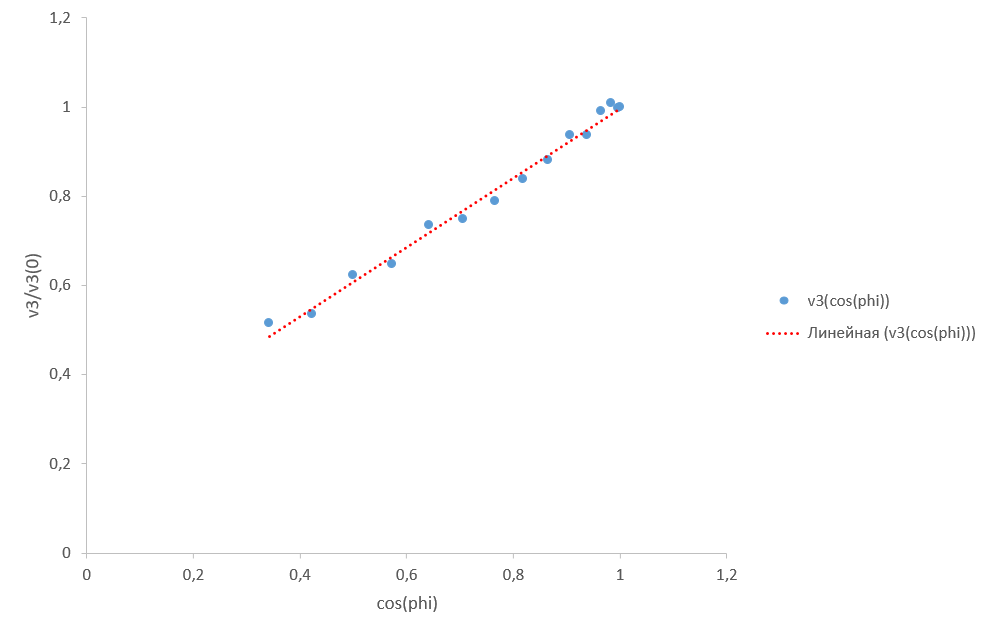
\includegraphics[width=0.9\textwidth]{gr1.png}
	\label{fig:boiler}
\end{figure}

Как видим, зависимость линейная, то есть лазерный луч действительно поляризован случайно.

11-12) Построим график зависимости видности от разности хода между пучками.

Данные можно найти в приложенной электронной таблице

\newpage

\begin{center}
	\Large $\nu_2(x)$
\end{center}

\begin{figure}[!h]
	\centering
	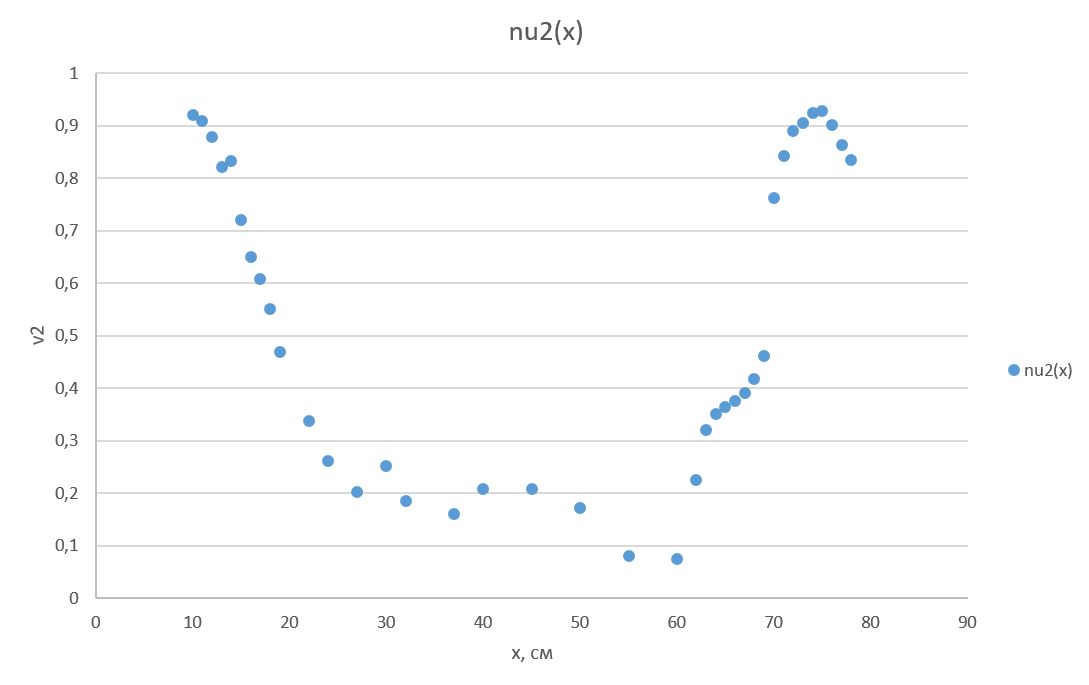
\includegraphics[width=0.9\textwidth]{gr2.png}
	\label{fig:boiler}
\end{figure}

На графике даже видны промежуточные горбы графика видности.

Максимумы графика $x_1 = 10 \pm 1$ см и $x_2 = 75 \pm 1$ см.

Тогда $L = \frac{x_2 - x_1}{2} = 33 \pm 1$ см.

И межмодовое расстояние $\nu_m = (4.3 \pm 0.2) \cdot 10^8$ Гц.

Оценим полуширину кривой. $l_{1/2} = 9$ см (первая кривая).

Полуширина диапазона частот $\Delta F = 1.2 \cdot \frac{c_0}{l_{1/2}} \approx 2 \cdot 10^9$ Гц.

А число мод $n = 1 + 1.2 \frac{L}{l_{1/2}} = 5 \pm 1$

\section{Вывод}

В работе была успешно исследована видность  интерференционной картины излучения гелий-неонового лазера, была определена его поляризация. Полученные зависимости согласуются с теоретическими.

\section{Ресурсы}

Расчет по МНК: метод-наименьших-квадратов.рф


\end{problem}
\end{document}